\documentclass[../../main.tex]{subfiles}

\begin{document}
\problem{8: Which field of the response message contains the IP address of \lstinline{www.ieee.org}?}
\begin{wts}
Which field of the response message contains the IP address of \lstinline{www.ieee.org}?
\end{wts}
\begin{proof}
    Consider the following Graphic.
    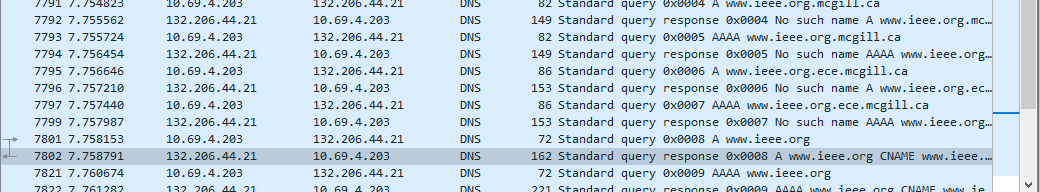
\includegraphics[width=\textwidth]{subfiles/images/308_Lab5_Part_1_PAGE0_0_Image20.png}
    \begin{itemize}
        \item - when a group of subnets are aggreated via route aggregation, can combine into a single bigger subnet.
        \item the number of allowed subnets within a given CIDR block is 2 more than the number of hosts. this is because the ‘slash’ prefix distinguishes between subnet number 0, and the supernet itself.
    \end{itemize}
\end{proof}

\end{document}